%\chapter{Joint Modeling of user latent behavior with semantic representation of text}
\chapter{Joint Modeling of user latent behavioral and content representations}
\label{chap:syntactic}
In this chapter, we jointly estimate user latent behavioral characteristics with improved text representations to improve offensive language prediction task.
Specifically, we estimate the abusive behavior of users, i.e., likelihood of posting an offensive content, on Twitter. Different from text representation approaches used in \Cref{chap:reliability} and \Cref{chap:induced}, we learn an improved text representation that is suitable to capture nuanced hate speech in text.
We further propagate user's abusive behavior through their social connections on Twitter to capture homophily in abusive user accounts. We finally show that combining the text and user representations can greatly improve offensive language prediction on future tweets \cite{hate}.

\section{Overview}
Abusive language usage in online social media is a grave issue that is affecting the interactions of users online. In a study conducted by Pew Research Center\footnote{http://www.pewinternet.org/2014/10/22/online-harassment/}, 40\% of adult Internet users have personally experienced harassment online, and 60\% have witnessed offensive name-calling. Social media websites, like Twitter and Facebook, allow users to report harassing content. However, due to the sheer volume of data, timely human curation of all reported content is not possible. Besides, there is also a need to filter these hateful content proactively. Therefore, there is an increased interest in automatic detection and moderation of hate speech in natural language processing \cite{waseem-hovy-2016}.

A typical definition of hate speech is as an \emph{attack} targeted towards a particular \emph{individual} or \emph{entity} belonging to
a protected group (protected group may include, but are not always limited to, religious, gender or racial minorities) \cite{elsherief2018hate}. Thus, hate speech identification can be cast as a relation extraction problem in which
the goal is to detect a "hate" or "attack" relation that links the speaker to a protected group (the object of the attack).

\begin{figure}[tbh]
    \centering
    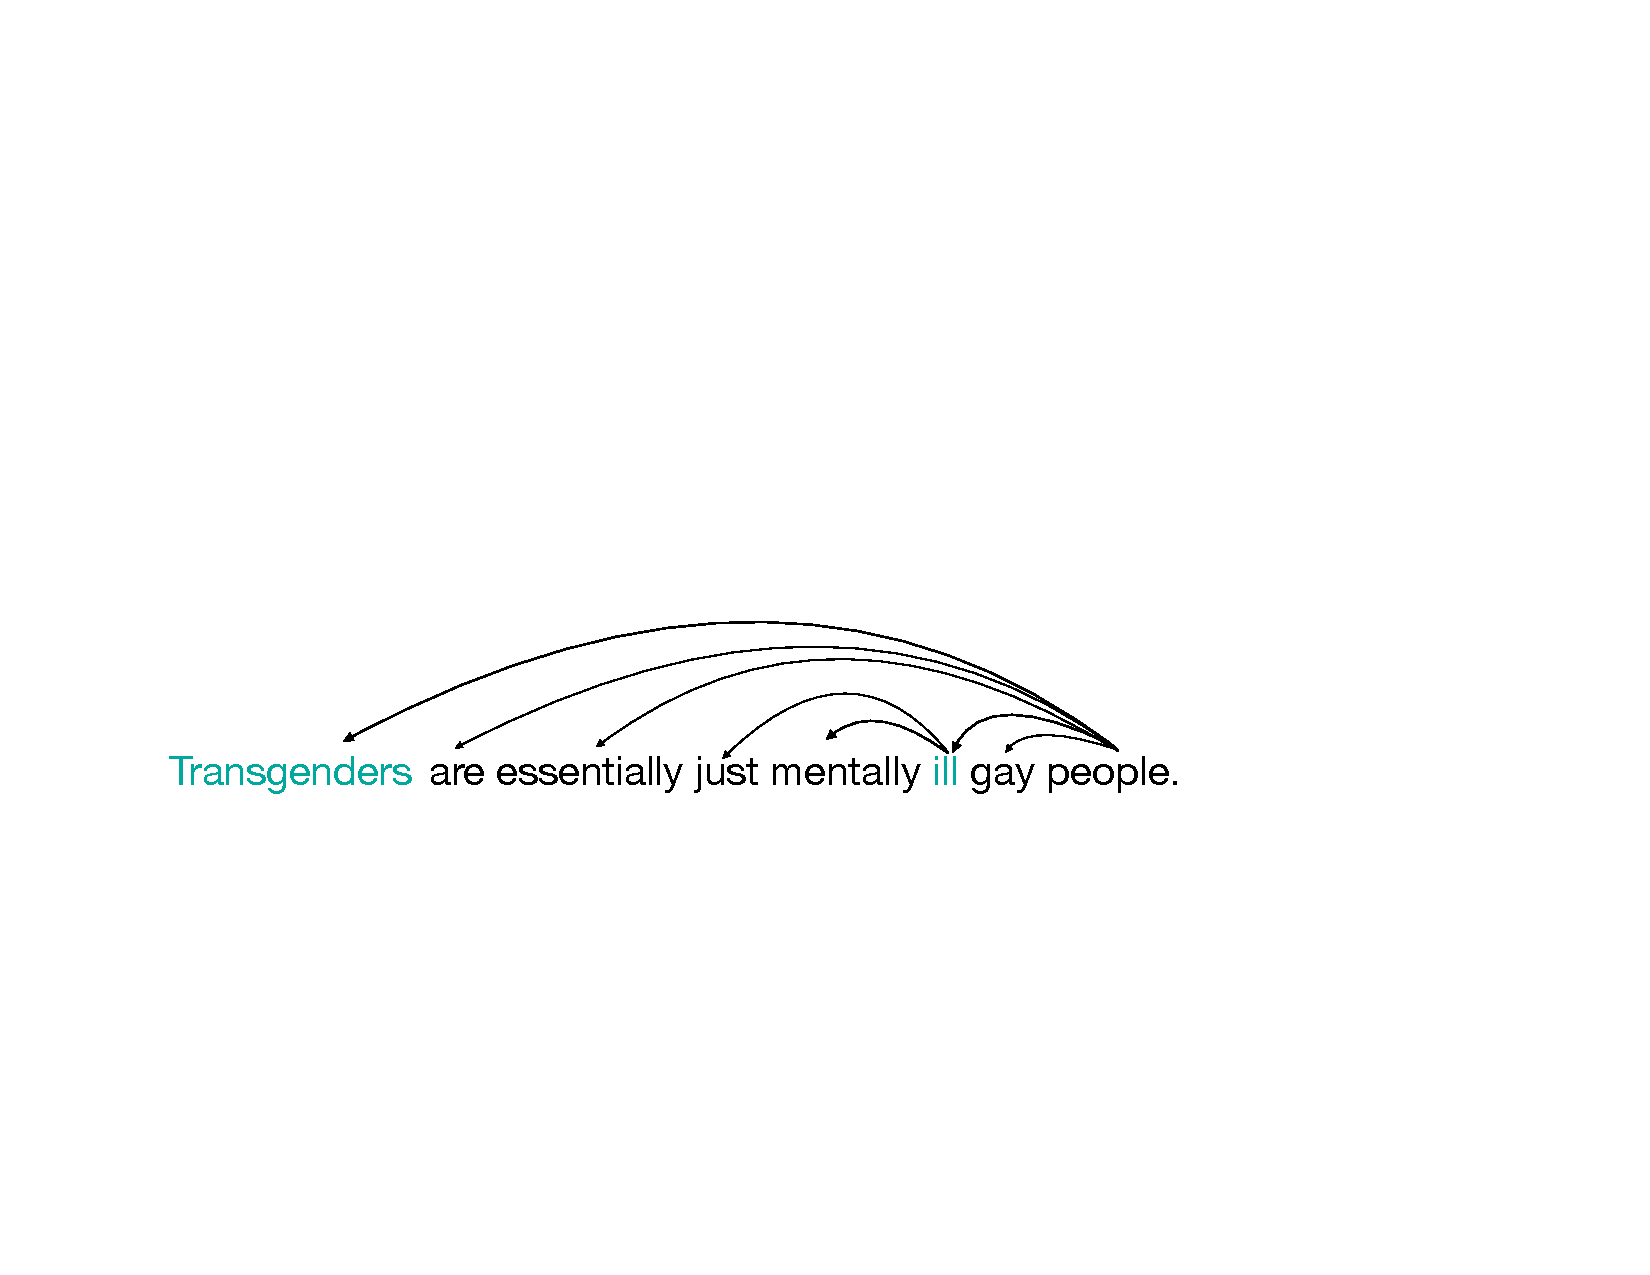
\includegraphics[scale=0.6]{figures/sample_key}
    \caption{Dependency parse for a sample hate tweet. The target \emph{Transgenders} is closer to the attack word, \emph{ill} in the parse tree. }
    \label{fig:parser}
\end{figure}


Current state-of-the-art methods in hate speech identification use either character or word n-gram features \cite{waseem-hovy-2016, davidson2017automated} or employ sequential deep learning models like CNN or LSTM \cite{ziqicnn, badjatiya2017deep}. However, these methods do not work well to capture long-range dependencies, for instance, in longer sentences with long clauses or complex scoping. Large pre-trained language models \cite{devlin2019bert} achieve very high accuracy after fine-tuning on supervised tasks. However, they typically learn pairwise attention between all words in the text and are thus computationally expensive. This makes them unfit to be used efficiently for real-time detection.

Recent work by \citet{clark2019does} analyzed attention mechanisms of the pre-trained BERT model and found that some of the attention heads are learning syntactic dependencies between words like direct objects of verbs, determiners of nouns, etc. A dependency parser also analyzes the grammatical structure of the sentence and returns the structure of syntactic dependence between words in the sentence. Recently, \citet{zhang-graph} used words in the dependency parse path between the subject and object of the sentence for extracting relations between them. They encoded the dependency parse graph using efficient graph convolution operations. Graph convolutional networks \cite{kipf2016semi} have been proposed for efficient convolutions over graph structured data. They are easy to parallelize and are computationally efficient.

However, a direct usage of \citet{zhang-graph}'s method is not straightforward because of the complexity of the possibilities for expressing the attack in text.
An attack may be expressed using explicit slurs or curses, as in: \emph{RT @USER: Stupid f*cking n*gger LeBron. You flipping jungle bunny monkey f*ggot}, or not, as in: \emph{Transgenders are essentially just mentally ill gay people}. In other instances, the attack can be \emph{implicit} like \emph{RT @USER: @USER every guy knows that the only thing that will make a woman happy is making any man a sandwich \#notsexist.}.
Moreover, the online text does not have annotated subject and object as in the benchmark datasets \cite{zhang-graph} and also often contains noisy text. However, parse structures can still be useful for capturing longer-range dependencies than sequential models (for instance, long clauses or complex scoping shown in these tweets). For instance, in Figure \ref{fig:parser}, the sequential distance between attack \emph{mentally ill} and target \emph{Transgenders} is five tokens, but while the distance in the parse tree is only two. Thus, we propose an adaption of the \cite{zhang-graph} model that learns a unified representation of text by encoding the whole dependency parse of the sentence. We later build a classifier based on this representation for identifying offensive language.

According to social influence theory \cite{social_influence}, users get influenced by their friends' behavior leading to user homophily \cite{homophily} (similar behavior) among connected users. Observable signals from social media can be taken as indicators of shared community membership.
\cite{mishra2019abusive} showed that most of the abusive behavior in their version of \citet{waseem-hovy-2016}'s dataset comes from a small set of densely connected users. They showed that incorporating user features along with linguistic features, can improve the hate classification task. We propose an extended version of our model that uses a user social graph in addition to the parser graph to learn extended embeddings.

%//Talk about our contributions and methods
In this work, we propose a classifier based on dependency graphical convolutional networks (DepGCN) to detect offensive language online. We tested our method on the benchmark Twitter hate speech datasets. Our model outperformed the current state-of-the-art \cite{waseem-hovy-2016, davidson2017automated} for offensive language detection and even strong baselines like fine-tuned BERT \cite{devlin2019bert}. We further propose a UserGCN model to incorporate the effect of social influence on user's abusive behavior. The UserGCN model learns a user's abusive behavior through a class prior and propagates this behavior through their social network. After merging the DepGCN with the UserGCN model, we achieve a new state-of-the-art on these benchmark datasets.
